\pdfoutput=1
\documentclass[11pt,french]{article}

% Remove the "review" option to generate the final version.
\usepackage{humanistica} % cf fichier `humanistica.sty`
\setlength\titlebox{7.3cm} % modifier la hauteur du `\maketitle`

% Standard package includes
\usepackage{times}
\usepackage{latexsym}
\usepackage[T1]{fontenc}
\usepackage[utf8]{inputenc}
\usepackage{microtype} % améliorations microtypographiques
\usepackage{babel}
\usepackage{csquotes}
\usepackage{epigraph}
\usepackage{subcaption}
\usepackage{authblk}
\renewcommand\Authands{, et }
\def\frenchtablename{Tableau} % les tables s'appellent `Tableau` dans les légendes

\usepackage{tikz}
\usetikzlibrary{shapes.geometric}

\definecolor{pastelviolet}{rgb}{0.8, 0.6, 0.79}
\definecolor{palepink}{rgb}{0.98, 0.85, 0.87}
\definecolor{plum}{rgb}{0.44, 0.11, 0.11}
\definecolor{lilac}{rgb}{0.8, 0.8, 1.0}
\definecolor{peachpuff}{rgb}{1.0, 0.85, 0.73}
\definecolor{lightpink}{rgb}{1.0, 0.71, 0.76}
\definecolor{pearl}{rgb}{0.94, 0.92, 0.84}
\definecolor{lightmauve}{rgb}{0.86, 0.82, 1.0}
\definecolor{cherryblossompink}{rgb}{1.0, 0.72, 0.77} 	
\definecolor{nadeshikopink}{rgb}{0.96, 0.68, 0.78}
\definecolor{pastelviolet}{rgb}{0.8, 0.6, 0.79}
\definecolor{moccasin}{rgb}{0.98, 0.92, 0.84}
\definecolor{persimmon}{rgb}{0.93, 0.35, 0.0}
\definecolor{electricpurple}{rgb}{0.75, 0.0, 1.0}
\definecolor{wildstrawberry}{rgb}{1.0, 0.26, 0.64}
\definecolor{outrageousorange}{rgb}{1.0, 0.43, 0.29}
\definecolor{darkterracotta}{rgb}{0.8, 0.31, 0.36}

\tikzstyle{act} = [%
	draw,%
	rectangle,%
	rounded corners=3pt,%
	minimum height=1cm,%
	fill=lilac,%
	draw=plum,%
	text centered,%
	text width=4cm%
]
\tikzstyle{db} = [%
	cylinder,%
	shape border rotate=90,%
	aspect=0.25,%
	fill=pastelviolet,%
	draw=plum,%
	text centered,%
	text width=4cm%
]
\tikzstyle{app} = [%
	trapezium,%
	trapezium left angle=70,%
	trapezium right angle=110,%
	minimum height=1cm,%
	fill=lightpink,%
	draw=plum,%
	text centered,%
	text width=3cm%
]
\tikzstyle{expl} = [%
	rectangle,%
	draw=plum,%
	fill=moccasin,%
	text centered,%
	text width=4cm%
]
\tikzstyle{arrow} = [%
	thick,%
	->,%
	>=stealth,%
	color=plum%	
]
\tikzstyle{doublearrow} = [%
	thick,%
	<->,%
	>=stealth,%
	color=plum,%
]

\title{\enquote{La marque du lieu} dans le \enquote{quartier Richelieu}: implications de la notion de lieu pour la modélisation et la visualisation d’un corpus iconographique, cartographique et textuel (Paris, 1750-1950)}


\author[1]{\textbf{Paul Kervegan}}
\author[1]{\textbf{Charlotte Duvette}}
\author[2]{\textbf{Loïc Jeanson}}
\author[1]{\textbf{Colin Prudhomme}}
\author[1]{\authorcr \textbf{Justine Gain}}
\author[1]{\textbf{Esther Dasilva}}
\author[1]{\textbf{Louise Baranger}}
\affil[1]{Institut national d'histoire de l'art \authorcr
\texttt{\{prenom.nom\}@inha.fr}}
\affil[2]{Université de Lausanne \authorcr
\texttt{\{prenom.nom\}@unil.ch}}

\begin{document}
\maketitle

\begin{abstract}
% abstract de l'abstract
À partir d'un corpus complexe (iconographique, cartographique, textuel) portant sur un quartier parisien (1750-1950), nous proposons de définir un élément à même de réunir, de modéliser et de représenter nos sources: le lieu. Celui-ci permet de faire converger les composantes spatiales et historiques de notre corpus. Il s'agit alors de montrer la manière dont le lieu est appréhendé d'un point de vue technique: de quelle manière il peut être modélisé, mais aussi comment il peut être représenté dans un modèle 3D historique. Enfin, nous présenterons la manière dont le lieu peut servir de moteur pour l'exploration et l'interaction avec le corpus sur une application Web. En définitive, nous souhaitons interroger la manière dont le lieu vient modifier notre rapport aux sources et à la technique, dans le cadre d'un projet en humanités numériques et en histoire de l'architecture.
\end{abstract}

\section*{Introduction}
\epigraph{
	Il serait indispensable, et […] pourtant presque impossible de restituer la ville à la fois dans l'espace et dans le temps. De l'agencement de la rue, du décor des façades au cours de l'histoire, on ne connaît jamais qu'un moment.
}{Françoise Boudon \citep{boudon_systeme_1977}}

Les projets numériques visant à restituer la ville, dans l'espace et dans le temps, doivent composer avec l'aspect insaisissable de son tissu urbain, en proie à des transformations quasi continues. Plusieurs projets, notamment autour des \enquote{Time Machine}, s'attachent néanmoins à proposer une forme de restitution de la ville par la production et l'analyse de données socio-historiques: des cartes et atlas historiques sont mis en relation avec de grands volumes de données issues d'annuaires et de documents administratifs OCRisés
\citep{khemakhem_fueling_2018,berenbaum_mining_2018,bell_automated_2020,di_leonardo_approche_2021,uchida_benchmark_2022}. Le programme de recherche \enquote{Richelieu. Histoire du quartier} expérimente une approche complémentaire : étudier et restituer un quartier parisien (1750-1950) à partir de trois types de corpus : cartographique, iconographique et textuel. L'objectif est de comprendre la ville, ses usages et ses transformations, aussi bien urbaines qu'architecturales, économiques ou sociales, à partir d'images numérisées issues de bibliothèques numériques d'institutions publiques. Les images montrant la ville, et celles qui y sont produites, sont spatialisées et systématiquement rattachées à un lieu. Il s'agit pour nous de développer une méthodologie numérique pour croiser et structurer des corpus de données hétérogènes, l'objectif final étant d'exposer ces corpus sur une application Web pour représenter l'évolution urbaine dans le temps et l'espace.

Cette approche de la restitution numérique d'un quartier parisien soulève plusieurs questions:

Pourquoi ces déterminations spatiales et historiques influencent-elles la production, la modélisation, la représentation de données? En quoi ces déterminations peuvent-elles être modélisées? Comment utiliser le lieu pour exposer spatialement l'iconographie relative à un quartier dans son contexte urbain? En quoi l'utilisation de bibliothèques numériques impacte-elle la constitution de corpus iconographiques et modifie l'approche d'historien$\cdot$ne$\cdot$s de l'art?

Après avoir présenté notre approche et le projet dans lequel s'inscrit notre réflexion (partie \ref{sec:I}), il s'agira de présenter la notion de lieu, telle que nous l'utilisons et l'avons modélisée dans le projet: le lieu est un objet complexe qui fait converger nos trois corpus (partie \ref{sec:II}). Nous présenterons enfin les implications techniques de cette notion de lieu dans la modélisation des données, leur production et leur représentation sur une application Web (partie \ref{sec:III}).

\section{Le quartier Richelieu, le projet Richelieu: une approche \textit{spatial turn}}
\label{sec:I}
Cette réflexion sur la notion de lieu s'inscrit dans le cadre du programme \href{https://quartier-richelieu.inha.fr}{\enquote{Richelieu. Histoire du quartier}}. \enquote{Quartier Richelieu} est un nom d'usage appliqué à un secteur de Paris dont la topographie est définie en fonction des espaces et des monuments marquant des étapes importantes dans la constitution de son périmètre géographique. La place des Victoires, le Palais-Royal, l'avenue de l'Opéra, et, au nord, la ceinture des grands boulevards, marqueur historique de la distinction entre Paris et ses anciens faubourgs (fig. \ref{fig:quartier} et \ref{fig:spatial}). Notre approche consiste à regarder la ville comme un lieu en constante évolution, dont chaque état est le résultat d'un processus lié aux usages de la société et aux réseaux personnels et professionnels qui en sous-tendent les transformations. En cela, nous nous inscrivons dans le courant du \textit{spatial turn} ou \enquote{tournant spatial} (\citealp[p. 15-16]{bodenhamer_potential_2010}; \citealp{ayers_turning_2010}).

\begin{figure}[h!]
	\centering
	\includegraphics[width=\columnwidth]{includes/image4.png}
	\caption{Le quartier Richelieu}
	\label{fig:quartier}
\end{figure}

Durant la première phase du projet (2018-2020), les almanachs, bottins et annuaires du commerce de Paris (1830-1922) ont été océrisés et traités par \textit{datamining} \citep{di_leonardo_repopulating_2019}. La seconde phase du projet, débutée en 2021, est consacrée à l’iconographie et à la cartographie du quartier, avec pour cas d’étude la rue Vivienne et la place de la Bourse. Il s’agit de constituer, par une analyse fine des sources, trois corpus: iconographique, cartographique et textuel. Cette approche, par l’iconographie et par le lieu, est problématique. Prendre le parti de reconstituer l’histoire d’un secteur, en partie à travers des images, permet de documenter des états disparus de la ville, mais contraint à manipuler des informations lacunaires. L’analyse iconographique, méthode de recherche issue de l’histoire de l’art \enquote{traditionnelle}, se heurte ici aux outils mis à disposition par les bibliothèques numériques à partir desquelles les corpus sont constitués. Ces trois corpus servent de base à une chaîne de traitement numérique (fig. \ref{fig:pipeline}):

\begin{itemize}
	\item Spatialiser les sources cartographiques dans un SIG.
	\item Réaliser une modélisation 3D de lieux centraux du quartier à partir de sources iconographiques.
	\item Constituer une base de données PostgreSQL enrichissant nos trois corpus (textuel, iconographique, cartographique) et leurs métadonnées.
	\item Exposer ces corpus spatialisés sur une application Web.
\end{itemize}

\section{Définir un lieu}
\label{sec:II}
La notion de lieu se révèle centrale dans notre projet, tant d’un point de vue théorique, dans l’étude du quartier, que dans la pratique pour produire et structurer une base relationnelle. Afin de rendre cette notion opératoire, nous en proposons une définition à partir de laquelle s’élabore notre chaîne de traitement.

Un lieu est un espace défini par une géométrie s’inscrivant dans une certaine continuité. Selon l’échelle d’étude, le lieu pourrait correspondre à une pièce d’un bâtiment, au bâtiment lui-même, à une parcelle cadastrale, etc. Dans notre projet, un lieu correspond généralement à une parcelle, sur laquelle peuvent être construits des bâtiments (e.g. le Palais de la Bourse), qu’il est possible de désigner par un nom d’usage (e.g. le Palais de Cristal), et par une ou plusieurs adresses (e.g. 39, rue Vivienne en 1860-1900, actuel 37, rue Vivienne). Pour nous, l’unité inchangée reste l’espace. C’est à travers l'espace que nous traçons une continuité entre les informations relatives aux lieux à travers le temps, les transformations urbaines, les évènements, les opérations foncières et immobilières ou encore des changements de numérotation des rues. En modélisant ces lieux successifs ou mitoyens, nous réunissons les représentations de la ville tout en discrétisant les étapes des modifications du quartier.

\section{Implications techniques de la notion de lieu dans la modélisation, la production et la visualisation des corpus}
\label{sec:III}
\subsection{Modéliser un lieu}

\begin{figure}[htp]
	\centering
	\tikz[node distance=1cm, scale=0.7, transform shape]{
		\node[act] (lieu) at (0,0) 
		{Lieu};
		\node[act] (addresse) at (3,-2.25) 
		{Addresses};
		\node[act] (carte) at (-3,-2.25) 
		{Représentations cartographiques};
		\node[act] (groupe) at (0,2.5) 
		{Groupement synchronique des évolutions d'un lieu dans le temps};
		\draw[arrow] (lieu) -- (addresse);
		\draw[arrow] (lieu) -- (carte);
		\draw[arrow] (lieu) -- (groupe);
	}
	\caption{Représentation (simplifiée) d'un lieu dans un modèle relationnel}
	\label{fig:model}
\end{figure}

Dans la constitution d’une base relationnelle, définir un lieu en théorie ne suffit pas: cet objet doit être modélisé de façon concrète. Nous le définissons comme un objet ayant une empreinte au sol (représentée en GeoJSON), une coordonnée et existant durant une période chronologique donnée: des bordures spatiales et temporelles. Ce lieu, représenté par une table SQL, est caractérisé à l’aide d’autres tables qui y sont liées (fig. \ref{fig:model}). L’adresse et la toponymie, évolutives, auxquelles sont associées le lieu, forment une autre table, ce qui permet de disjoindre le lieu de son appellation. Le lieu est également distinct de sa représentation cartographique : représenter les métadonnées des plans cadastraux de parcelles sur une table à part permet à un seul lieu d’être représenté par différents plans. Ces trois objets (lieu, toponymie, cartographie) sont tous définis pour un moment donné; les évolutions d’un lieu dans le temps doivent alors être modélisées. Une dernière table relie donc tous les moments d’un lieu entre eux, de façon synchronique. En caractérisant un lieu par plusieurs objets de nature différente, il devient possible d’étudier celui-ci dans le temps et dans l’espace. En prévision du partage de données ouvertes aux formats du Web sémantique (API au format JSON-LD), le modèle de données partiellement présenté ci-dessus s’aligne également sur des standards de métadonnées (DublinCore) et des protocoles interopérables (IIIF).

\subsection{Du SIG à la modélisation 3D: méthodologies pour étudier et représenter l'évolution d'un lieu}
Notre hypothèse est qu’en faisant cohabiter des représentations du quartier en 2D et 3D, nous pouvons restituer pleinement la spatialité du corpus iconographique. C’est pourquoi une modélisation 3D de notre premier secteur d’étude -- la place de la Bourse -- est réalisée à partir d'un relevé par lasergrammétrie (fig. \ref{fig:laser}). Des sources historiques (représentations de façades sur des gravures, dessins, photos) sur plusieurs périodes (1830-1850-1880-1900) sont croisées avec ce relevé pour créer un modèle historique de l’espace public et architectural avec Blender. 

Ce processus est le début d’une réflexion sur la manière de représenter différentes couches temporelles d’un monument, afin de retranscrire ses évolutions historiques. Il s'appuie sur une étude attentive des sources iconographiques. Il s'agit d'abord de développer une méthodologie numérique pour évaluer leur qualité documentaire, en fonction de la technique utilisée (gravure, photographie...) et de leur précision. Il est ensuite nécessaire de spatialiser ces sources dans un SIG (fig. \ref{fig:pdv}), ce qui demande de reconstituer l'évolution du parcellaire aux alentours de la place de la Bourse. Pour réaliser un modèle 3D historique, il est donc nécessaire de mener une analyse computationnelle du quartier, de son découpage parcellaire et de ses représentations.

\subsection{Mobiliser le lieu pour explorer un corpus complexe sur le Web}
Forts d’une méthode et de données articulées par cette notion de lieu, nous interrogeons et expérimentons les possibilités numériques d’exploration de notre corpus au travers d’une application Web. Cette présentation permet de démontrer les moyens pensés, les déambulations souhaitées dans les données, qui seules nous permettent de visualiser le quartier au gré de ses transformations. Ces moyens relèvent de la sémantique graphique, mais également du design à proprement parler. Il doit faire du lieu un moyen d’explorer les trois corpus. Par cette déambulation entre documents iconographiques, représentation cartographique, modélisation 3D et focus historiques, nous voulons donner à voir le quartier, expliquer ses changements en donnant un accès direct et contextualisé aux sources à partir desquelles nous travaillons. 

%%%%%%%%%%%%%%%%% BIBLOGRAPHIE %%%%%%%%%%%%%%%%%
% ATTENTION: SI ON A DES ERREURS DE COMPILATION, C'EST PARCE QUE
% LA CHAÎNE DE COMPILATION EST MAL FAITE: IL FAUT FAIRE
% pdflatex => biber => pdflatex => pdflatex
%
% => solution: en ligne de commande, compiler avec `biber` le
% fichier `.aux`: 
% `biber ./{filename}.aux`
\bibliography{includes/humanistica.bib}



%%%%%%%%%%%%%%%%% ANNEXES %%%%%%%%%%%%%%%%%
\appendix
\section*{Annexes}
\begin{itemize}
	\item \textbf{Figure \ref{fig:pipeline}}: chaîne de traitement des corpus.
	\item \textbf{Figure \ref{fig:spatial}}: extrait de corpus spatialisé sur une carte du quartier.
    \item \textbf{Figure \ref{fig:laser}}: relevé par lasergrammétrie de la place de la Bourse
    \item \textbf{Figure \ref{fig:pdv}}: spatialisation des points de vue depuis lesquels est représentée la place de la Bourse dans un SIG
\end{itemize}

\clearpage
% figure*: environnement permettant l'image pleine page malgré les colonnes
\begin{figure*}
	\centering
	\tikz[node distance=1cm, scale=0.67, transform shape]{
		\node[act] (etude) at (0,5)
		{Constitution de corpus};
		\node[act] (sig) at (-10,5)
		{SIG: spatialisation des sources cartographiques};
		
		\node[expl] (carto) at (0,2) 
		{Métadonnées du corpus cartographique (CSV)};
		\node[expl] (icono) at (-5,2) 
		{Métadonnées du corpus iconographique (CSV)};
		\node[expl] (bottins) at (5,2) 
		{Données extraites des bottins et annuaires (CSV)};
		
		\node[act] (tosql) at (0,-0.5)
		{Enrichissement et transformation en SQL};
		\node[act] (sig-extract) at (-10,-0.5)
		{Extraction d'informations spatiales};
		\node[act] (3D) at (10, 5)
		{Modélisation 3D à partir d'un relevé photogrammétrique et de sources historiques};
		
		\node[db] (sql) at (0,-4)
		{Base de données contenant les informations issues des 3 corpus (PostgreSQL)};
		\node[db] (3Dmodel) at (10,-4)
		{Modèle 3D historique};
		
		\node[app] (backend) at (0, -7)
		{Application \textit{backend}};
		\node[app] (frontend) at (-4, -9)
		{Application \textit{frontend}};
		\node[app] (api) at (4, -9)
		{API pour le partage de données brutes};
		
		\draw[arrow] (etude) -- (carto);
		\draw[arrow] (etude) -- (icono);
		\draw[arrow] (etude) -- (bottins);
		\draw[arrow] (etude) -- (sig);
		\draw[arrow] (etude) -- (3D);
		\draw[arrow] (3D) -- (3Dmodel);
		\draw[arrow] (sig) -- (sig-extract);
		\draw[arrow] (sig-extract) -- (tosql);
		\draw[arrow] (carto) -- (tosql);
		\draw[arrow] (icono) -- (tosql);
		\draw[arrow] (bottins) -- (tosql);
		\draw[arrow] (tosql) -- (sql);
		\draw[doublearrow] (sql) -- (backend);
		\draw[arrow] (backend) -- (frontend);
		\draw[arrow] (backend) -- (api);
		\draw[doublearrow] (backend) -- (10,-7) -- (3Dmodel);
	}
	\caption{Chaîne de traitement des trois corpus, depuis leur constitution jusqu'à leur exposition}
	\label{fig:pipeline}
\end{figure*}

\clearpage
\begin{figure*}[!p]
	\centering
	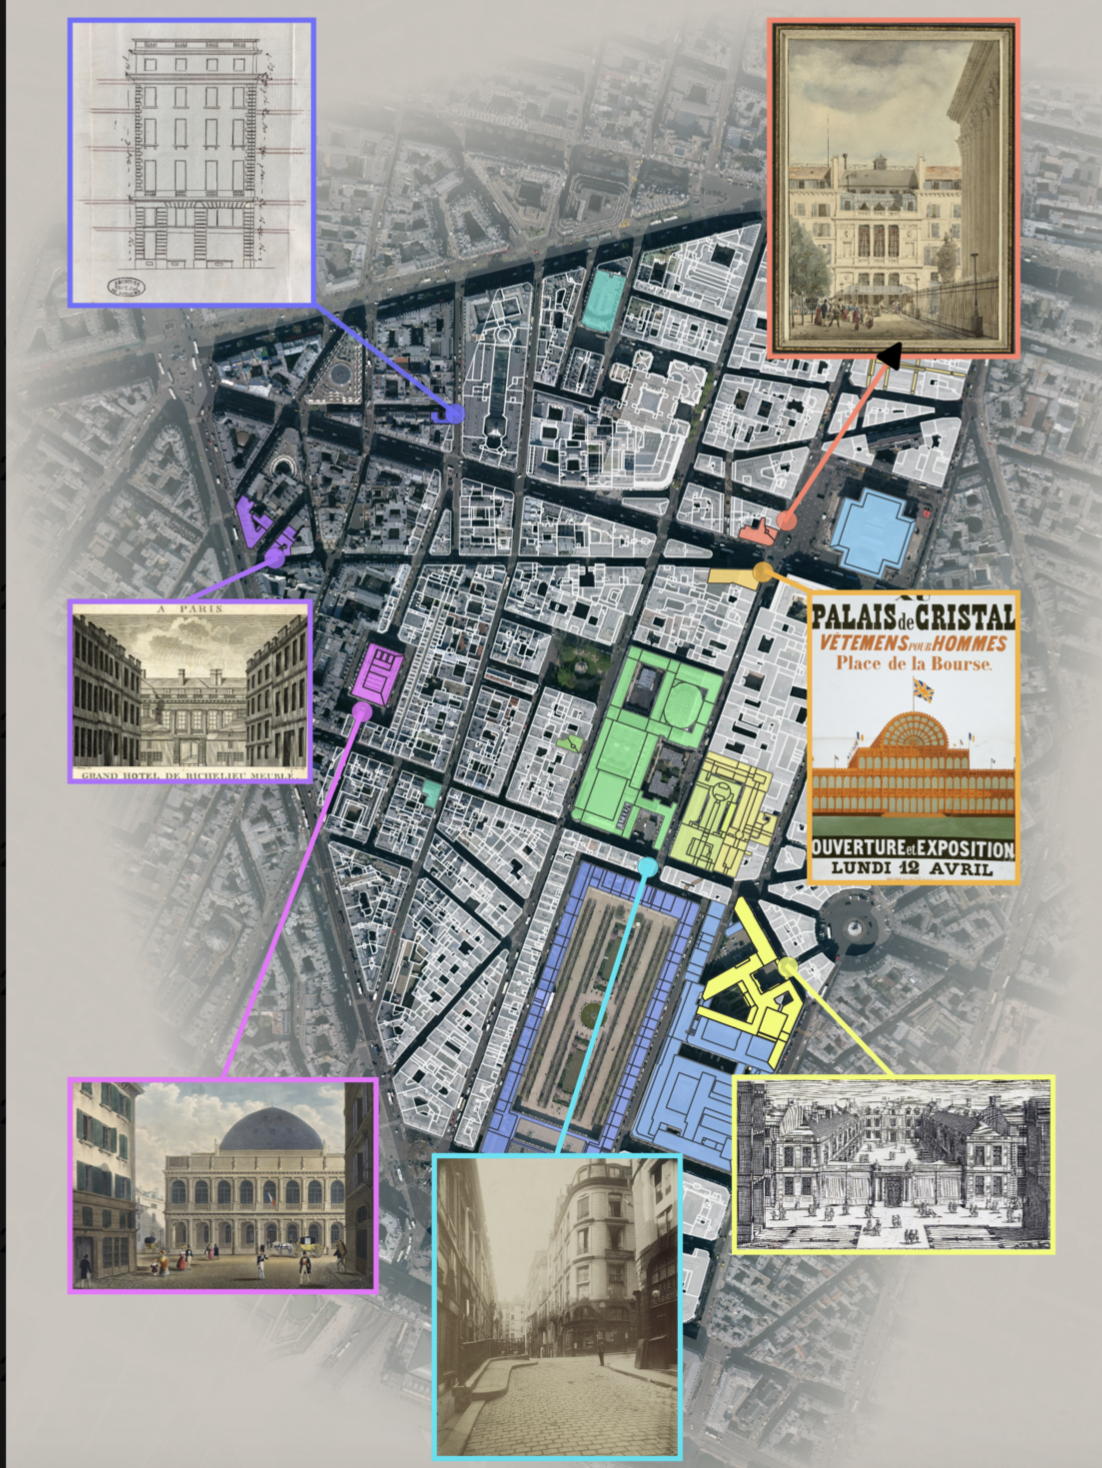
\includegraphics[width=\textwidth]{includes/image2.png}
	\caption{Iconographie spatialisée représentant le quartier Richelieu}
	\label{fig:spatial}
\end{figure*}

\clearpage
\begin{figure*}[!p]
 \centering
 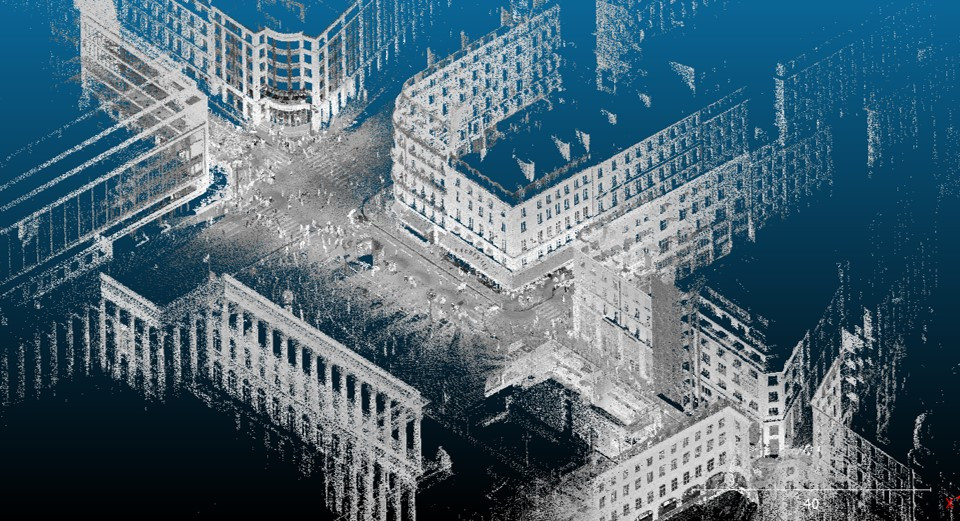
\includegraphics[width=\textwidth]{includes/lasergrammetrie.jpg}
 \caption{Relevé par lasergrammétrie de la place de la Bourse réalisée par le programme \enquote{Richelieu. Histoire du quartier} le 12 mars 2023 avec PLEMO3D (Sorbonne Université, Centre André Chastel)}
 \label{fig:laser}
\end{figure*}

\clearpage
\begin{figure*}[!p]
 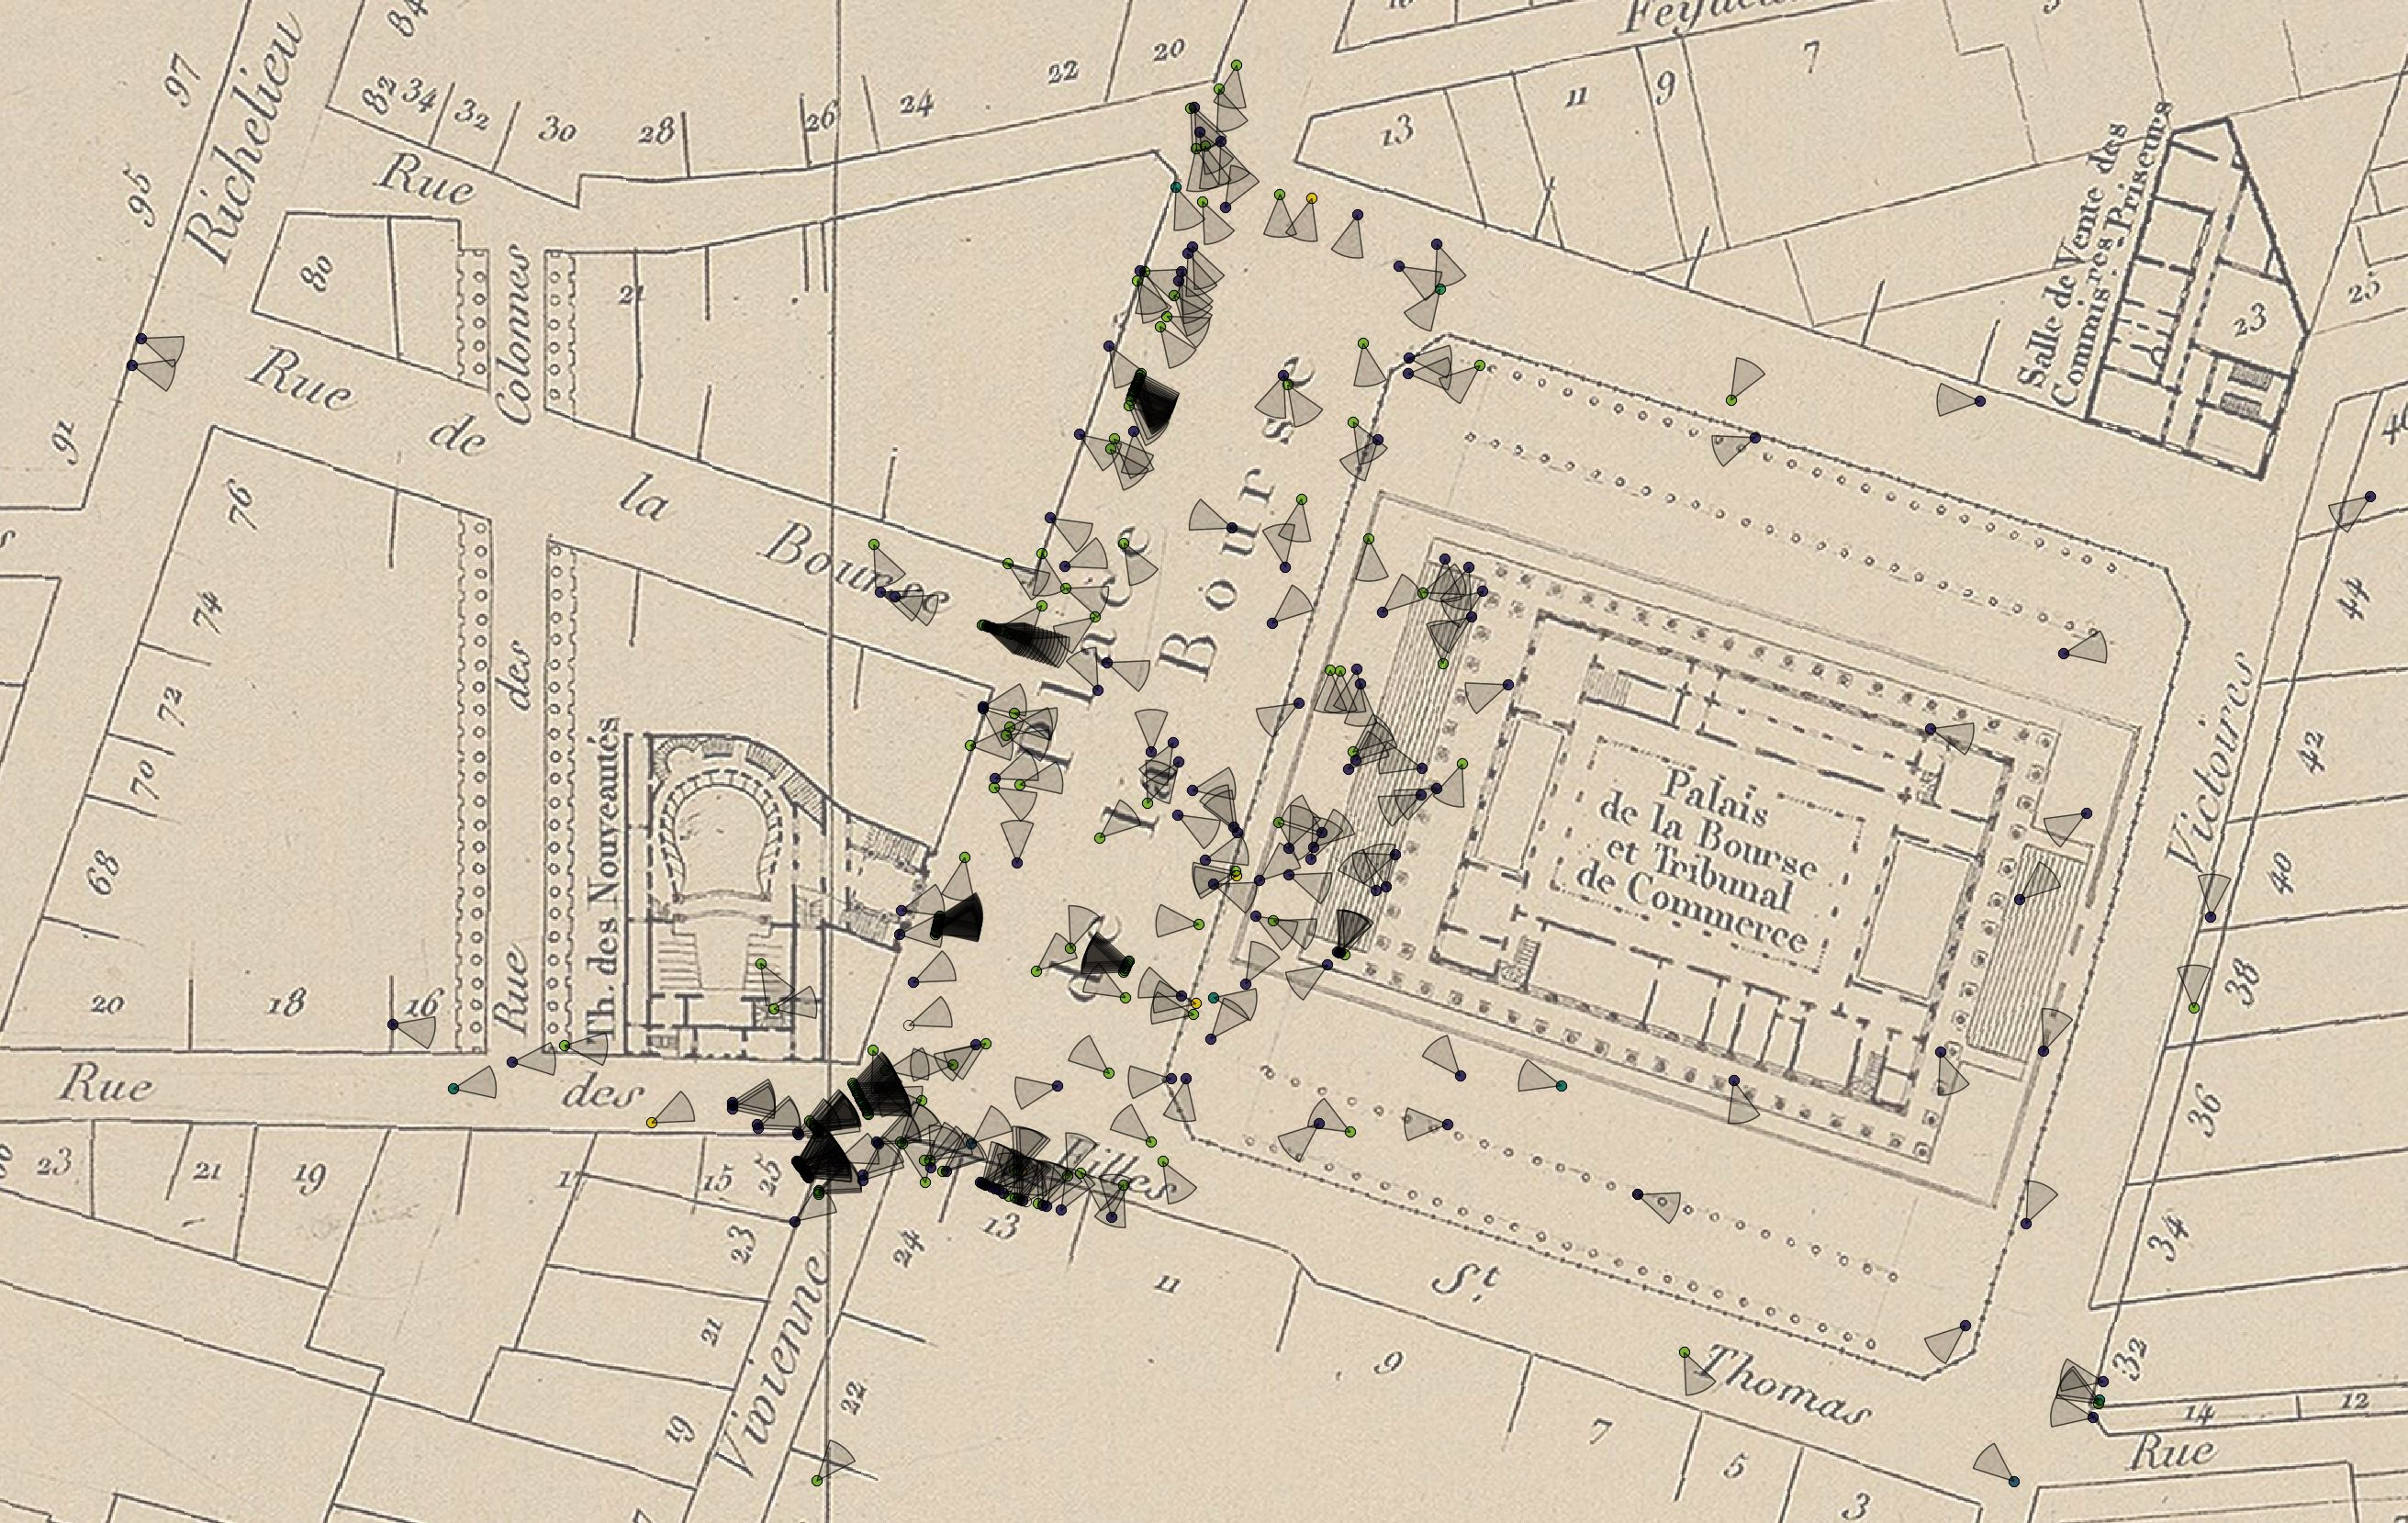
\includegraphics[width=\textwidth]{includes/pdv.jpg}
 \caption{Spatialisation dans un SIG des points de vue depuis lesquels est représentée la place de la Bourse}
 \label{fig:pdv}
\end{figure*}

\end{document}
